\documentclass[8pt]{beamer}
\usefonttheme[onlymath]{serif}
\newcommand\bmale{\fontsize{6}{7.2}\selectfont}
\newcommand\male{\fontsize{8}{7.2}\selectfont}
\newcommand\normalne{\fontsize{10}{7.2}\selectfont}
\newcommand\duze{\fontsize{12}{7.2}\selectfont}
\setbeamertemplate{caption}{\raggedright\insertcaption\par}

\graphicspath{{commons/}}

 \AtBeginSection[]{
   \begin{frame}
   \vfill
 \centering
   \begin{beamercolorbox}[sep=8pt,center,shadow=true,rounded=true]{title}
     \usebeamerfont{title}\insertsectionhead\par%
   \end{beamercolorbox}
   \vfill
   \end{frame}
 }

\mode<presentation>
{
  \usetheme{CambridgeUS}
  \usecolortheme{beaver}
}
\usepackage{tikz}
\usetikzlibrary{shapes,arrows,positioning}
\tikzstyle{block} = [rectangle, draw, fill=blue!20, rounded corners, align = center, minimum height=2.5cm, minimum width=4cm]
\tikzstyle{line} = [draw, thin, ->, >=stealth]
\tikzstyle{cloud} = [draw, ellipse,fill=red!20, node distance=3cm,    minimum height=2em]

\usepackage{pgfplots}
\usepackage{ulem}
\usepackage{tabto}
\usepackage[]{algorithm2e}
\usepackage{bm}
\usepackage{lmodern}
\usepackage[T1]{fontenc}
\usepackage[polish]{babel}
\usepackage[utf8]{inputenc}
\usepackage{pgfplots}
\usepackage{textcomp}

\DeclareMathOperator*{\argmin}{argmin}
\DeclareMathOperator*{\argmax}{argmax}
\selectlanguage{polish}

\title[Kraków, 2018] % (optional, use only with long paper titles)
{Introduction to Transportation Planning}

\subtitle
{Route-choice, fixed point, assignment}

\author[dr in\.z. Rafa\l{} Kucharski] % (optional, use only with lots of authors)
{dr in\.z. Rafa\l{} Kucharski\inst{1}}

\institute[] % (optional, but mostly needed)
{
  \inst{1}%
  Katedra System\'{o}w Transportowych\\
  Politechnika Krakowska
 }


\date[KST, L-2, WIL, PK] % (optional, should be abbreviation of conference name)
{Krak\'{o}w, 2018}

\pgfdeclareimage[height=1cm]{university-logo}{commons/ZSK}
 \logo{\pgfuseimage{university-logo}}

\AtBeginSubsection[]
%{
%  \begin{frame}<beamer>{Outline}
%    \tableofcontents[currentsection,currentsubsection]
%  \end{frame}
%}
%\beamerdefaultoverlayspecification{<+->}


\begin{document}

\begin{frame}
  \titlepage
\end{frame}


\begin{frame}{Fixed-point problem in transportation}{Limited-capacity}
Travel time is variable and changes with the demand.
\begin{block}{Waiting time}
How long will I travel across the Aleje?
\end{block}
\begin{equation*}
t_a=f(q_a)
\end{equation*}
\begin{center}
 \begin{tikzpicture}
% Draw the log-normal distribution curve
\draw[blue,smooth,thick] plot[id=f1,domain=0.001:3,samples=50]
({\x,{((1+(\x/3)^2)}});
% Draw the x-axis
\draw[->,black] (0,0) -- (3,0) node[anchor = south west] {$q_a$};
% Draw the y-axis
\draw[->,black] (0,0) -- (0,2) node[anchor = south east] {$t_a$};
\end{tikzpicture}
\end{center}
Travel time \textbf{non-linearly} grows with number of cars at Aleje.
\end{frame}


\begin{frame}{Fixed-point problem in transportation}{}
\begin{equation*}
q_z^n=f(q_z^{n-1})
\end{equation*}
\begin{enumerate}
\item how many drivers will select Aleje today (day $n$)? 
\item it depends on how satisfied they were from their decision yesterday (day $n-1$).
\item if number of drivers who selected Aleje today equals the number of drivers who selected Aleje yesterday - we are in the fixed-point - the system \textbf{stabilized/equilibrated}.
\item it also means that travel time at Aleje is exaclty, like it was yesterday, and exactly like it was expected by the drivers who selected Aleje.
\end{enumerate}
\end{frame}

\begin{frame}{Fixed-point problem in transportation}{Convergence}
	\begin{equation*}
		q_z^n=f(q_z^{n-1})
	\end{equation*}
	\begin{center}
		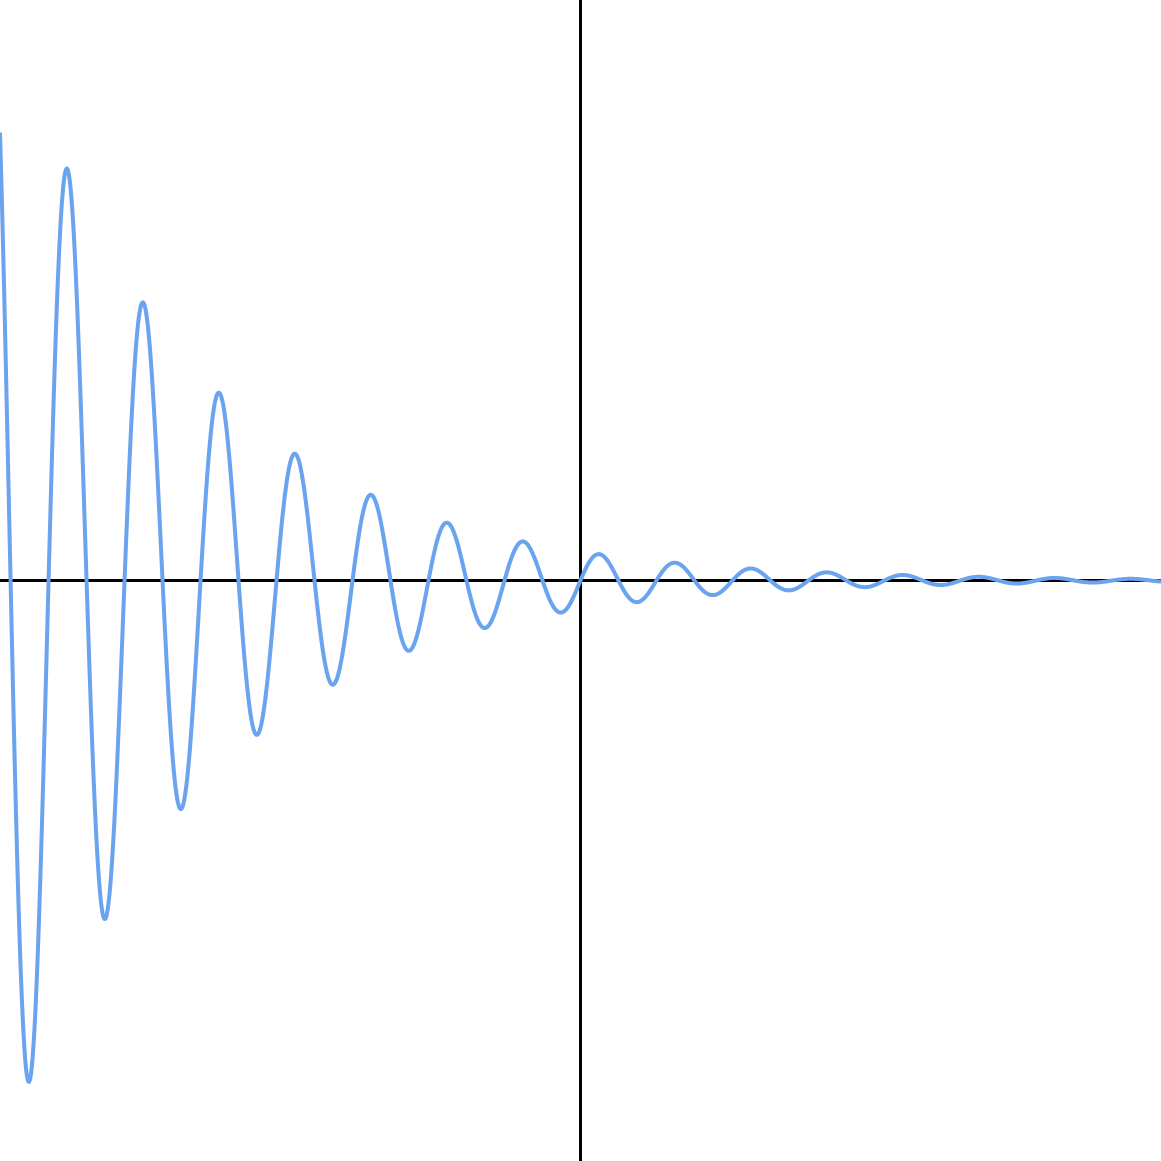
\includegraphics[height=5cm]{Harmonic} 
	\end{center}
\end{frame}

\begin{frame}{Fixed-point problem in transportation}{Convergence}
	\begin{equation*}
		q_z^n=f(q_z^{n-1})
	\end{equation*}
	Days (iterations):
	\begin{description}
		\item[1st] users on shortest paths - congested shortest paths
		\item[2-$\infty$] users try to avoid congestion and find better path, which are however not as good as expected
		\item[$\infty$] User Equilibrium
	\end{description}
	\begin{block}{User Equilibrium}
		\begin{enumerate}
			\item The journey times on all the routes actually used are equal and less than those which would be experienced by a single vehicle on any unused routes
			\item 	user-optimized equilibrium is reached when no user may lower his transportation cost through unilateral action.
		\end{enumerate}	
	\end{block}
\end{frame}


\section{Path choice}
\begin{frame}{Road network path choice}
For the transport network illustrated below let's determine the traffic flows on the bridge (dashed) and resulting travel time ($t_a$)
Numbers in zones show demand, i.e. number of cars willing to travel from the zone to the destination (factory) at the bottom. 
\\ Let's  assume all links are of equal length and their free flow travel time is 1min. Let's further assum
\begin{enumerate}
\item unlimited capacity of all arcs
\item bridge capacity ($Q_a$) is 500 vehicles/hour, other links have unkimited capacity. TO estimate travel time use this BPR formula: $t_a=t_a^0 \cdot (1+ (q_a / Q_a)^2)$. Give approximated value close to Wardop conditions.
\end{enumerate}
\end{frame}



\begin{frame}{Road network path choice}{numerical example}
A: inifnite capacity on all roads
\begin{center}
\begin{tikzpicture}[darkstyle/.style={circle,draw,fill=gray!40,minimum size=20}]
\draw (6,4)--(6,2) ;
\draw (8,4)--(8,2) ;
\draw (10,4)--(10,2) ;
\draw (0,2)--(10,2) ;
\draw (0,2)--(0,0) ;
\draw (0,0)--(8,0) ;
\draw (8,0)--(8,2) ;
\draw (8,0)--(8,-2) ;
       \node [darkstyle]  (1) at (6,4) {1000}; 
       \node [darkstyle]  (2) at (8,4) {300};
       \node [darkstyle]  (3) at (10,4) {700};
       \node [style={circle,draw,fill=gray!10,minimum size=20}]  (1) at (8,-2) {Cel}; 
       \node [style={circle,draw,fill=gray!0,minimum size=1}]  (1) at (0,0) {}; 
       \node [style={circle,draw,fill=gray!0,minimum size=1}]  (1) at (2,0) {};
       \node [style={circle,draw,fill=gray!0,minimum size=1}]  (1) at (4,0) {};
       \node [style={circle,draw,fill=gray!0,minimum size=1}]  (1) at (6,0) {};   
       \node [style={circle,draw,fill=gray!0,minimum size=1}]  (1) at (8,0) {}; 
       \node [style={circle,draw,fill=gray!0,minimum size=1}]  (1) at (0,2) {}; 
       \node [style={circle,draw,fill=gray!0,minimum size=1}]  (1) at (2,2) {};
       \node [style={circle,draw,fill=gray!0,minimum size=1}]  (1) at (4,2) {};  
       \node [style={circle,draw,fill=gray!0,minimum size=1}]  (1) at (6,2) {}; 
       \node [style={circle,draw,fill=gray!0,minimum size=1}]  (1) at (8,2) {}; 
       \node [style={circle,draw,fill=gray!0,minimum size=1}]  (1) at (10,2) {}; 
       
       
\end{tikzpicture}
\end{center}
\end{frame}


\begin{frame}{Road network path choice}{numerical example}
B: bridge capacity ($Q_a$) is 500 vehicles/hour, other links have unkimited capacity. TO estimate travel time use this BPR formula: $t_a=t_a^0 \cdot (1+ (q_a / Q_a)^2)$. Give approximated value close to Wardop conditions.
\begin{center}
\begin{tikzpicture}[darkstyle/.style={circle,draw,fill=gray!40,minimum size=20}]
\draw (6,4)--(6,2) ;
\draw (8,4)--(8,2) ;
\draw (10,4)--(10,2) ;
\draw (0,2)--(10,2) ;
\draw (0,2)--(0,0) ;
\draw (0,0)--(8,0) ;
\draw [thick, dashed] (8,0)--(8,2) ;
\draw (8,0)--(8,-1) ;
       \node [darkstyle]  (1) at (6,4) {1000}; 
       \node [darkstyle]  (2) at (8,4) {300};
       \node [darkstyle]  (3) at (10,4) {700};
       \node [style={circle,draw,fill=gray!10,minimum size=20}]  (1) at (8,-1) {Cel}; 
       \node [style={circle,draw,fill=gray!0,minimum size=1}]  (1) at (0,0) {}; 
       \node [style={circle,draw,fill=gray!0,minimum size=1}]  (1) at (2,0) {};
       \node [style={circle,draw,fill=gray!0,minimum size=1}]  (1) at (4,0) {};
       \node [style={circle,draw,fill=gray!0,minimum size=1}]  (1) at (6,0) {};   
       \node [style={circle,draw,fill=gray!0,minimum size=1}]  (1) at (8,0) {}; 
       \node [style={circle,draw,fill=gray!0,minimum size=1}]  (1) at (0,2) {}; 
       \node [style={circle,draw,fill=gray!0,minimum size=1}]  (1) at (2,2) {};
       \node [style={circle,draw,fill=gray!0,minimum size=1}]  (1) at (4,2) {};  
       \node [style={circle,draw,fill=gray!0,minimum size=1}]  (1) at (6,2) {}; 
       \node [style={circle,draw,fill=gray!0,minimum size=1}]  (1) at (8,2) {}; 
       \node [style={circle,draw,fill=gray!0,minimum size=1}]  (1) at (10,2) {}; 
       
       
\end{tikzpicture}
\end{center}
\end{frame}

\section{Path choices}
\begin{frame}{Shortest paths}{distance}
\begin{figure}\begin{center}
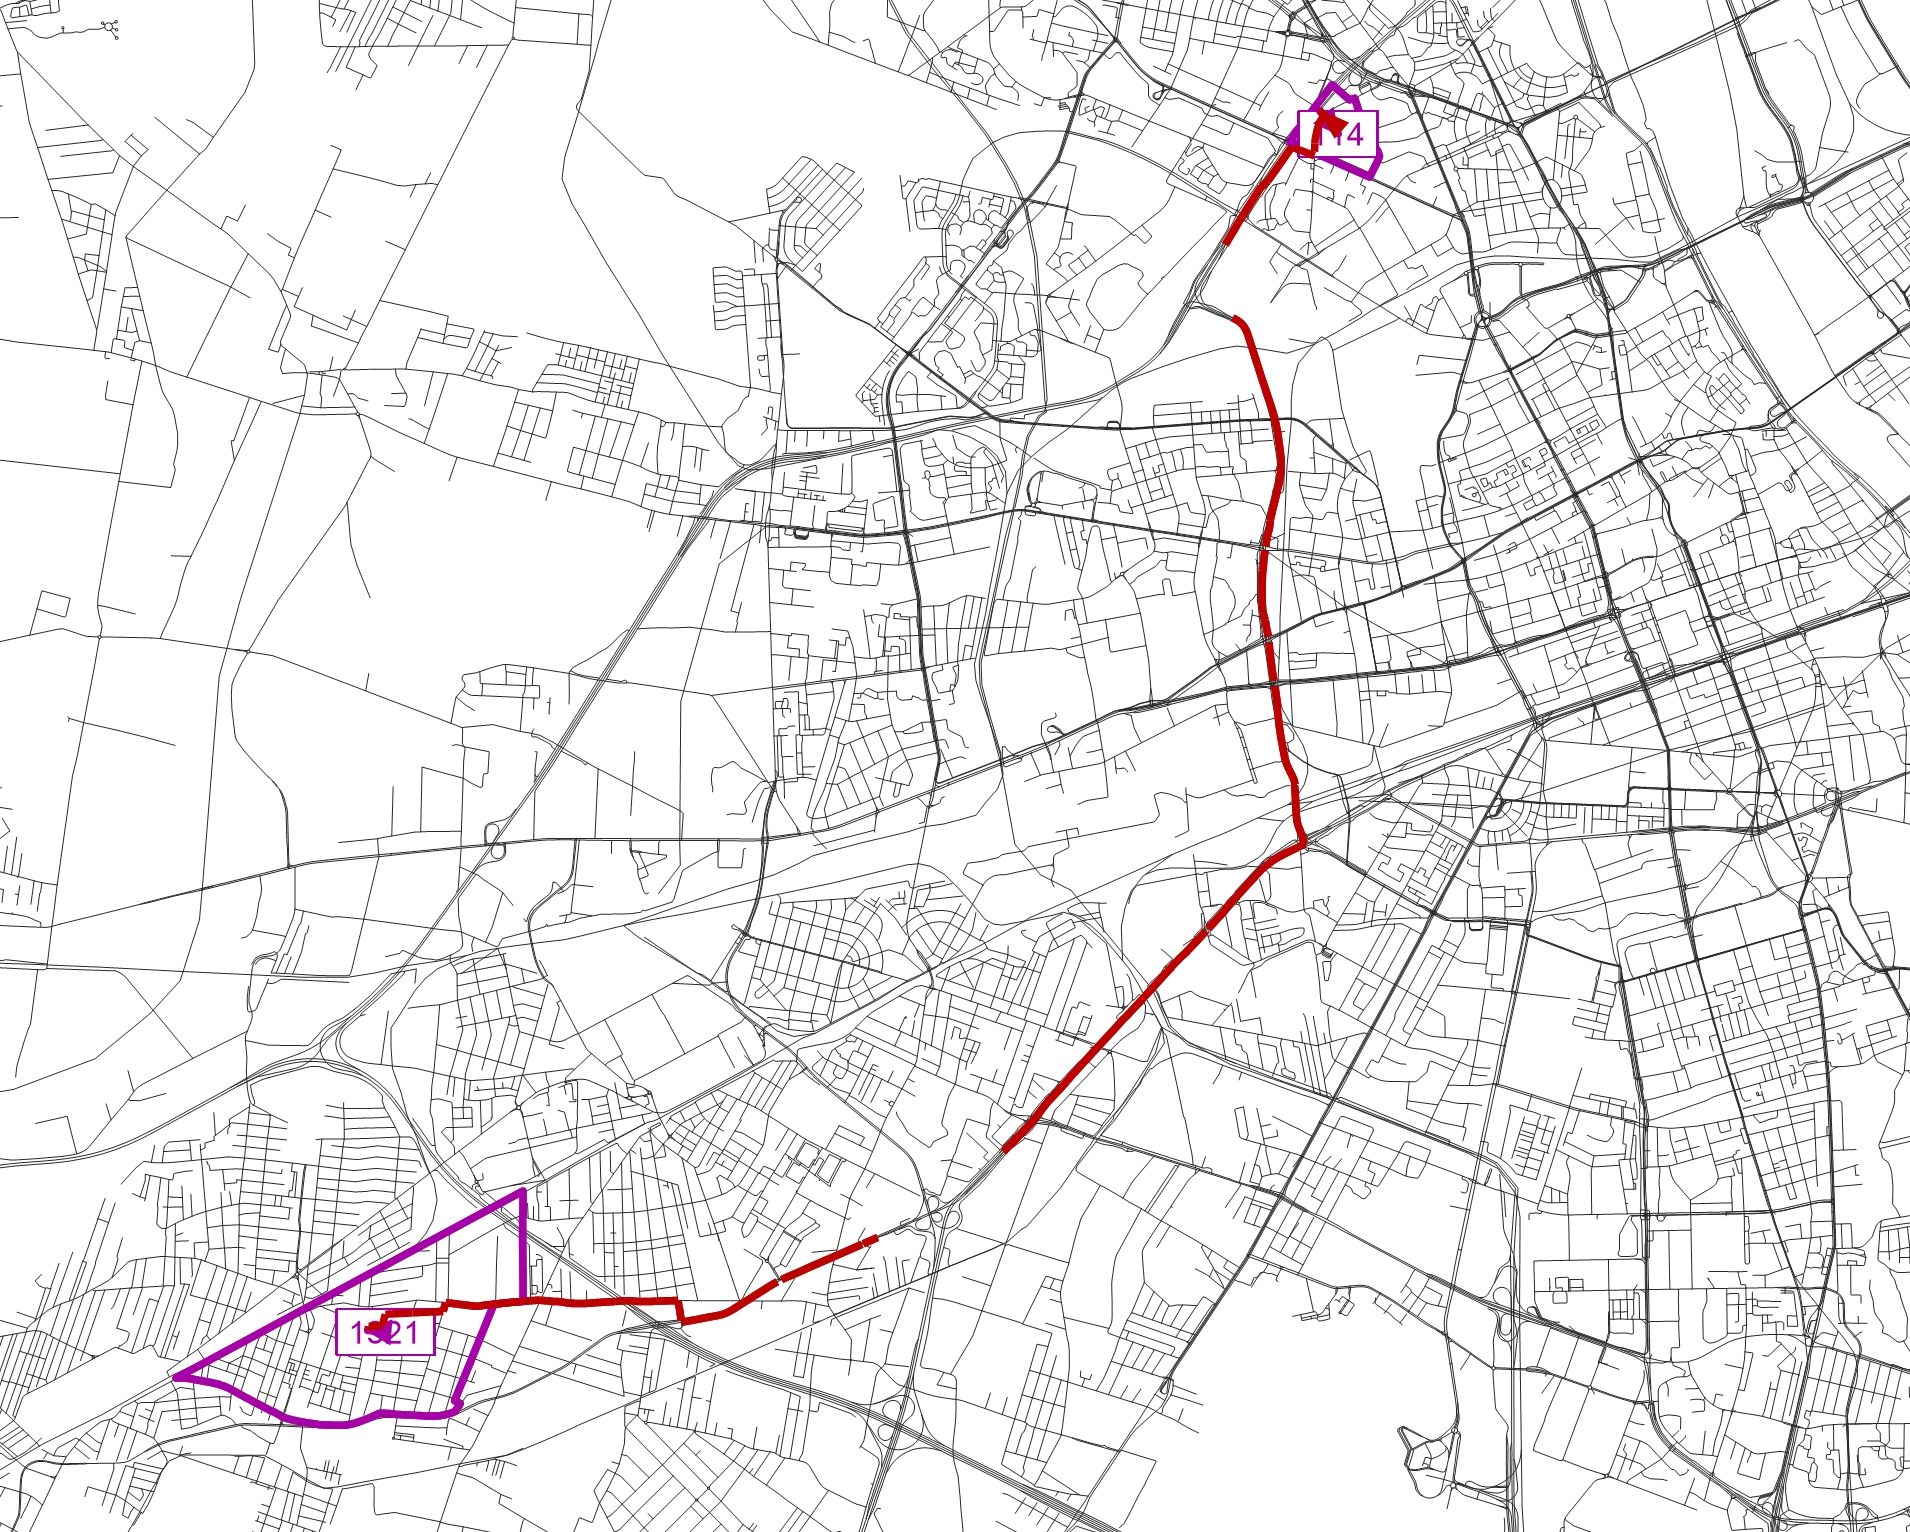
\includegraphics[width=0.8\textwidth]{path_dist}
 \end{center}  \end{figure} 
\end{frame}

\begin{frame}{Shortest paths}{time}
\begin{figure}\begin{center}
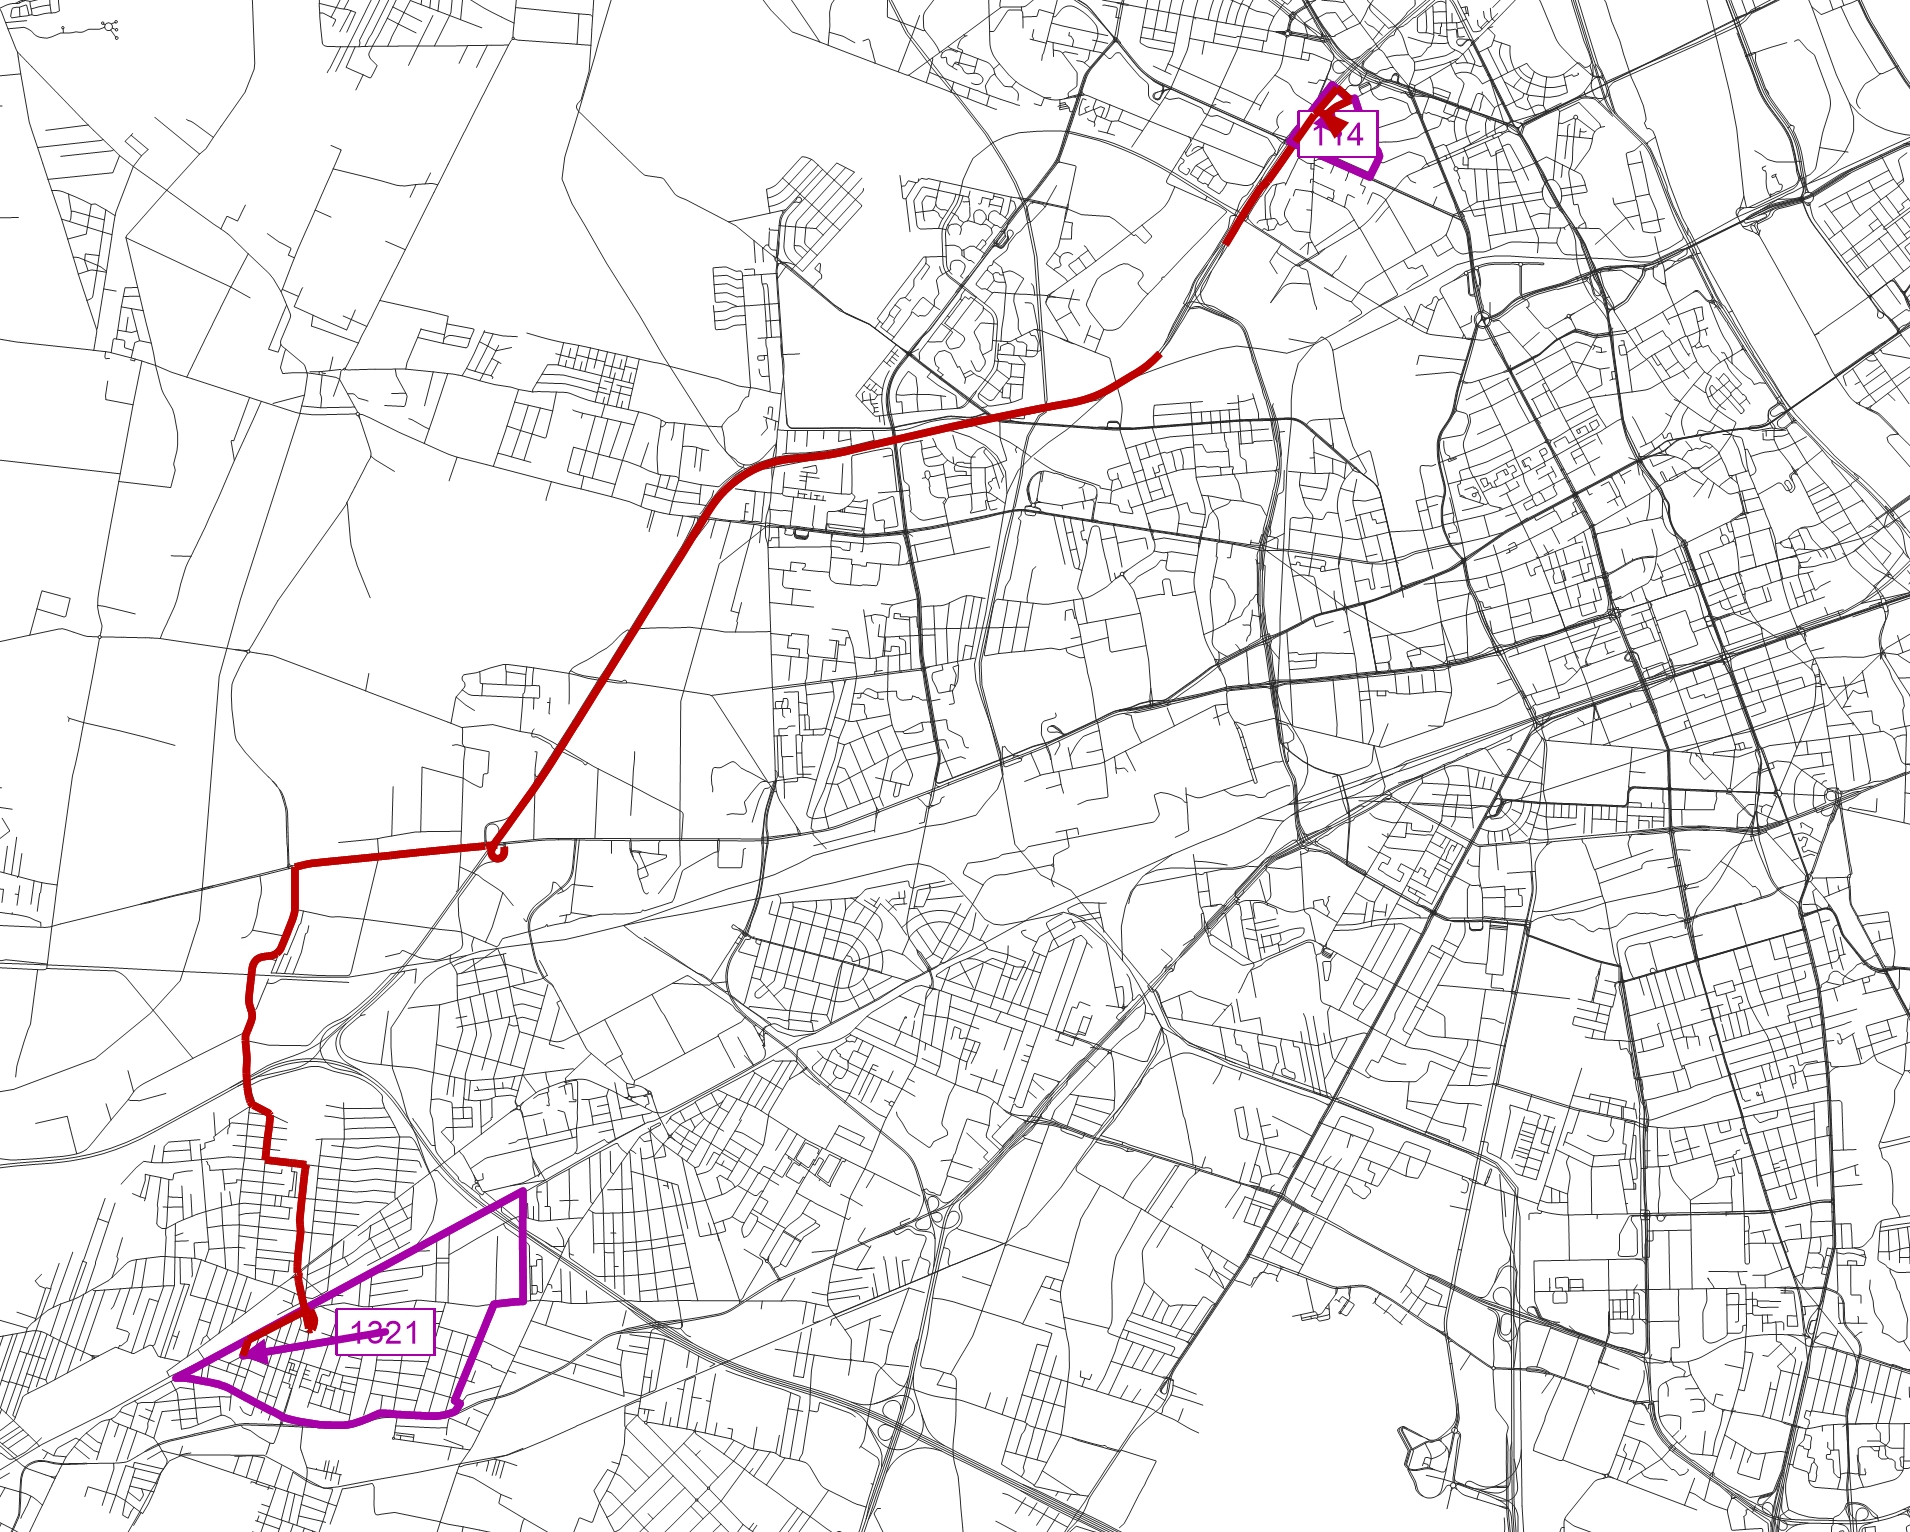
\includegraphics[width=0.8\textwidth]{path_time}
 \end{center}  \end{figure} 
\end{frame}

\begin{frame}{Shortest paths}{Congested time}
\begin{figure}\begin{center}
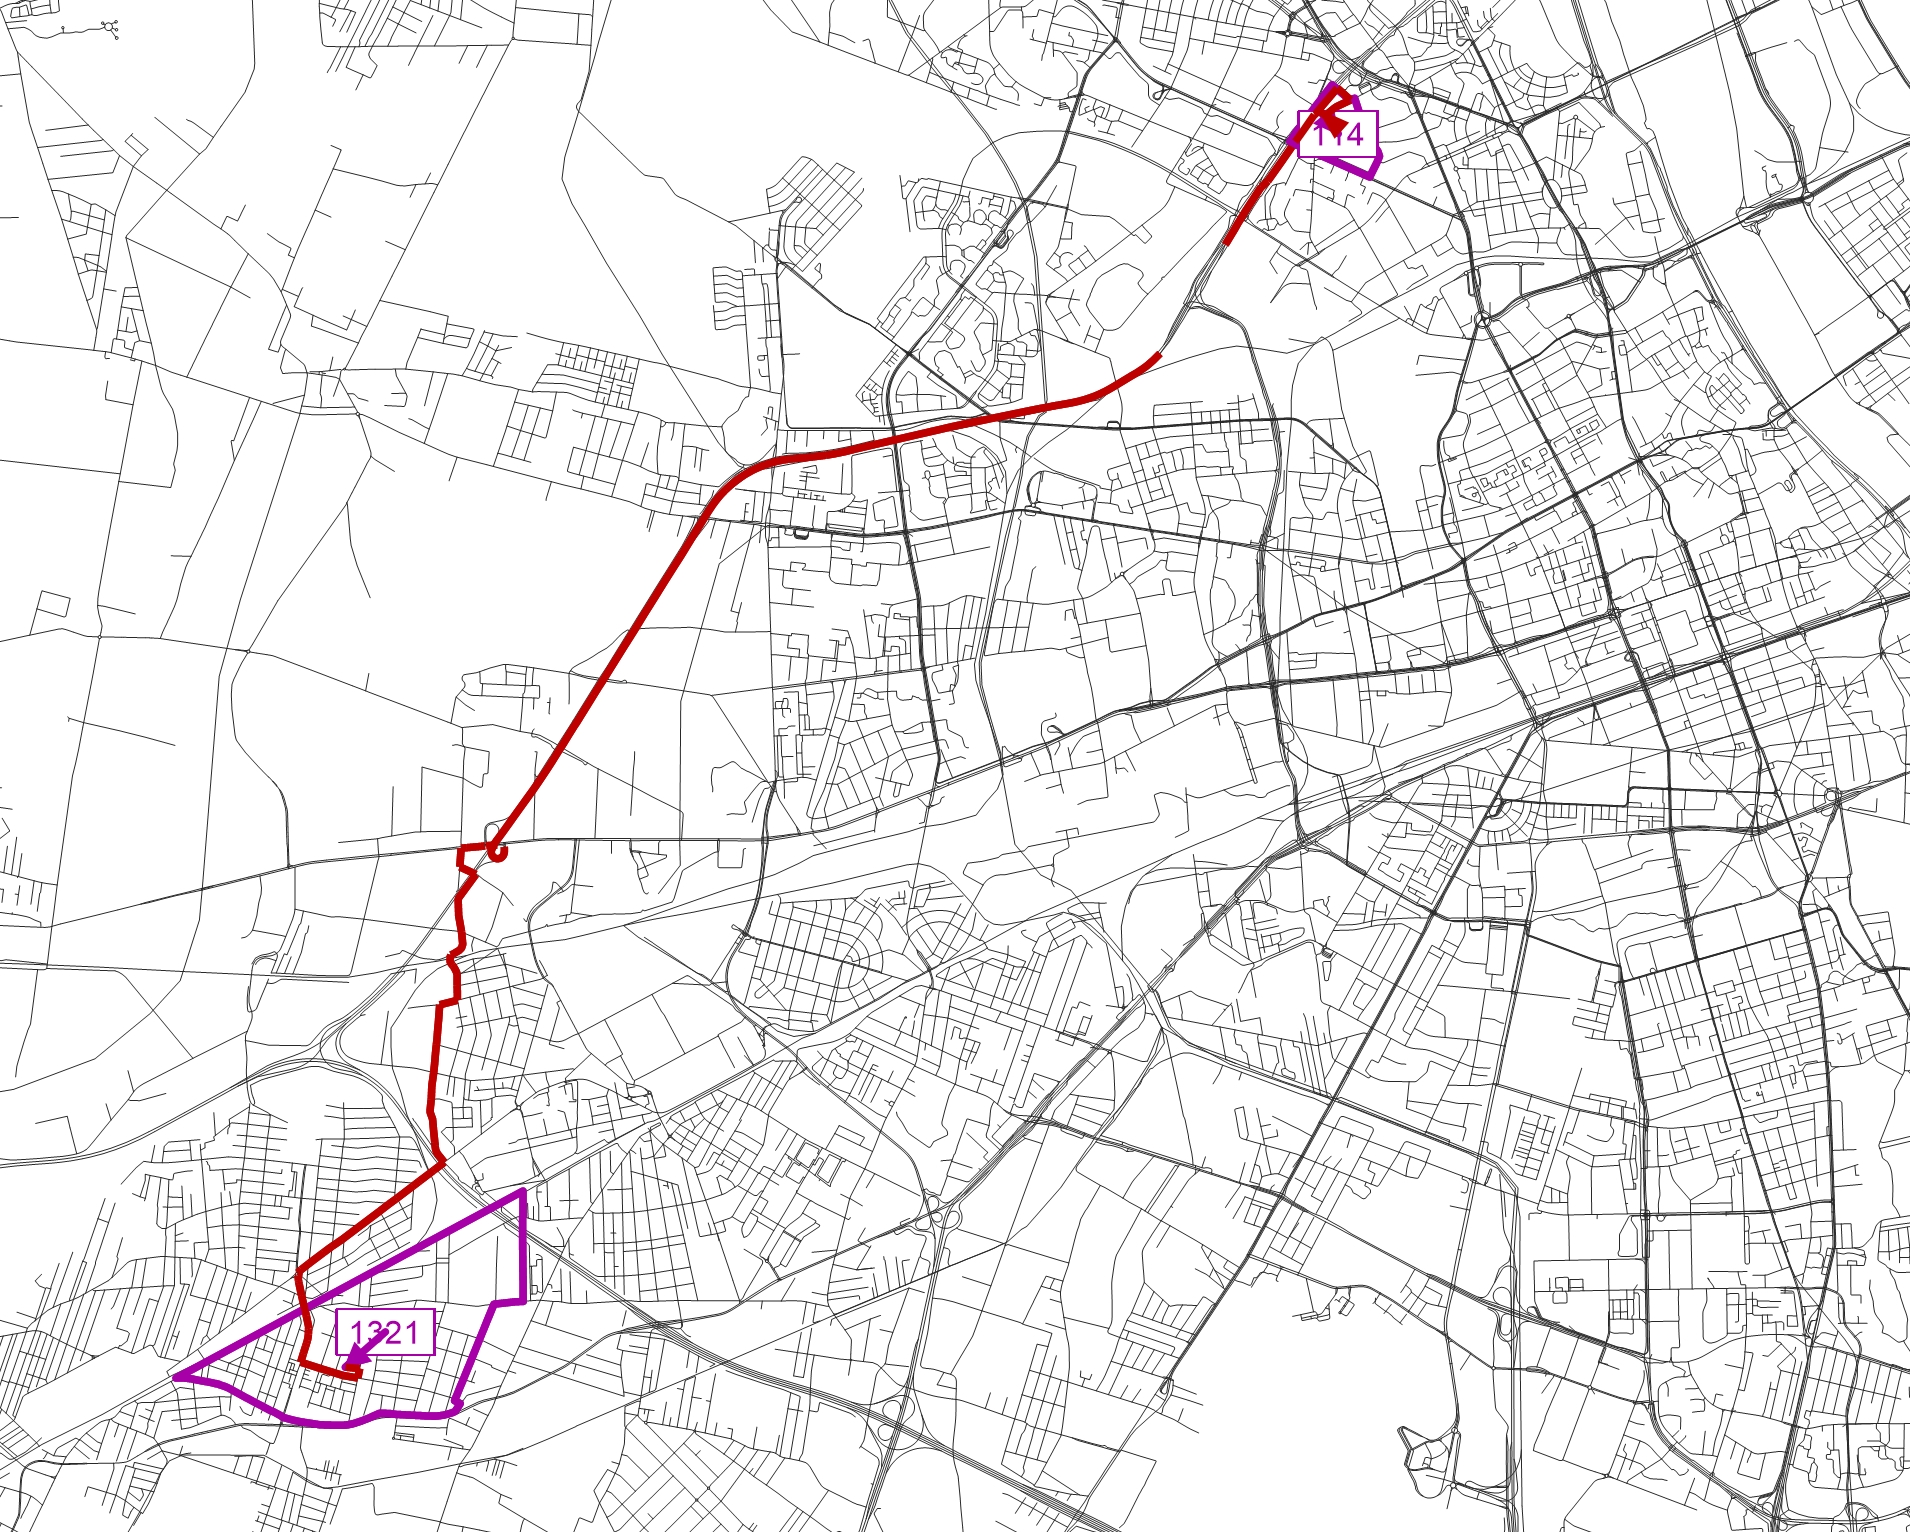
\includegraphics[width=0.8\textwidth]{path_jam}
 \end{center}  \end{figure} 
\end{frame}

\begin{frame}{Shortest paths}{Transit AM peak}
\begin{figure}\begin{center}
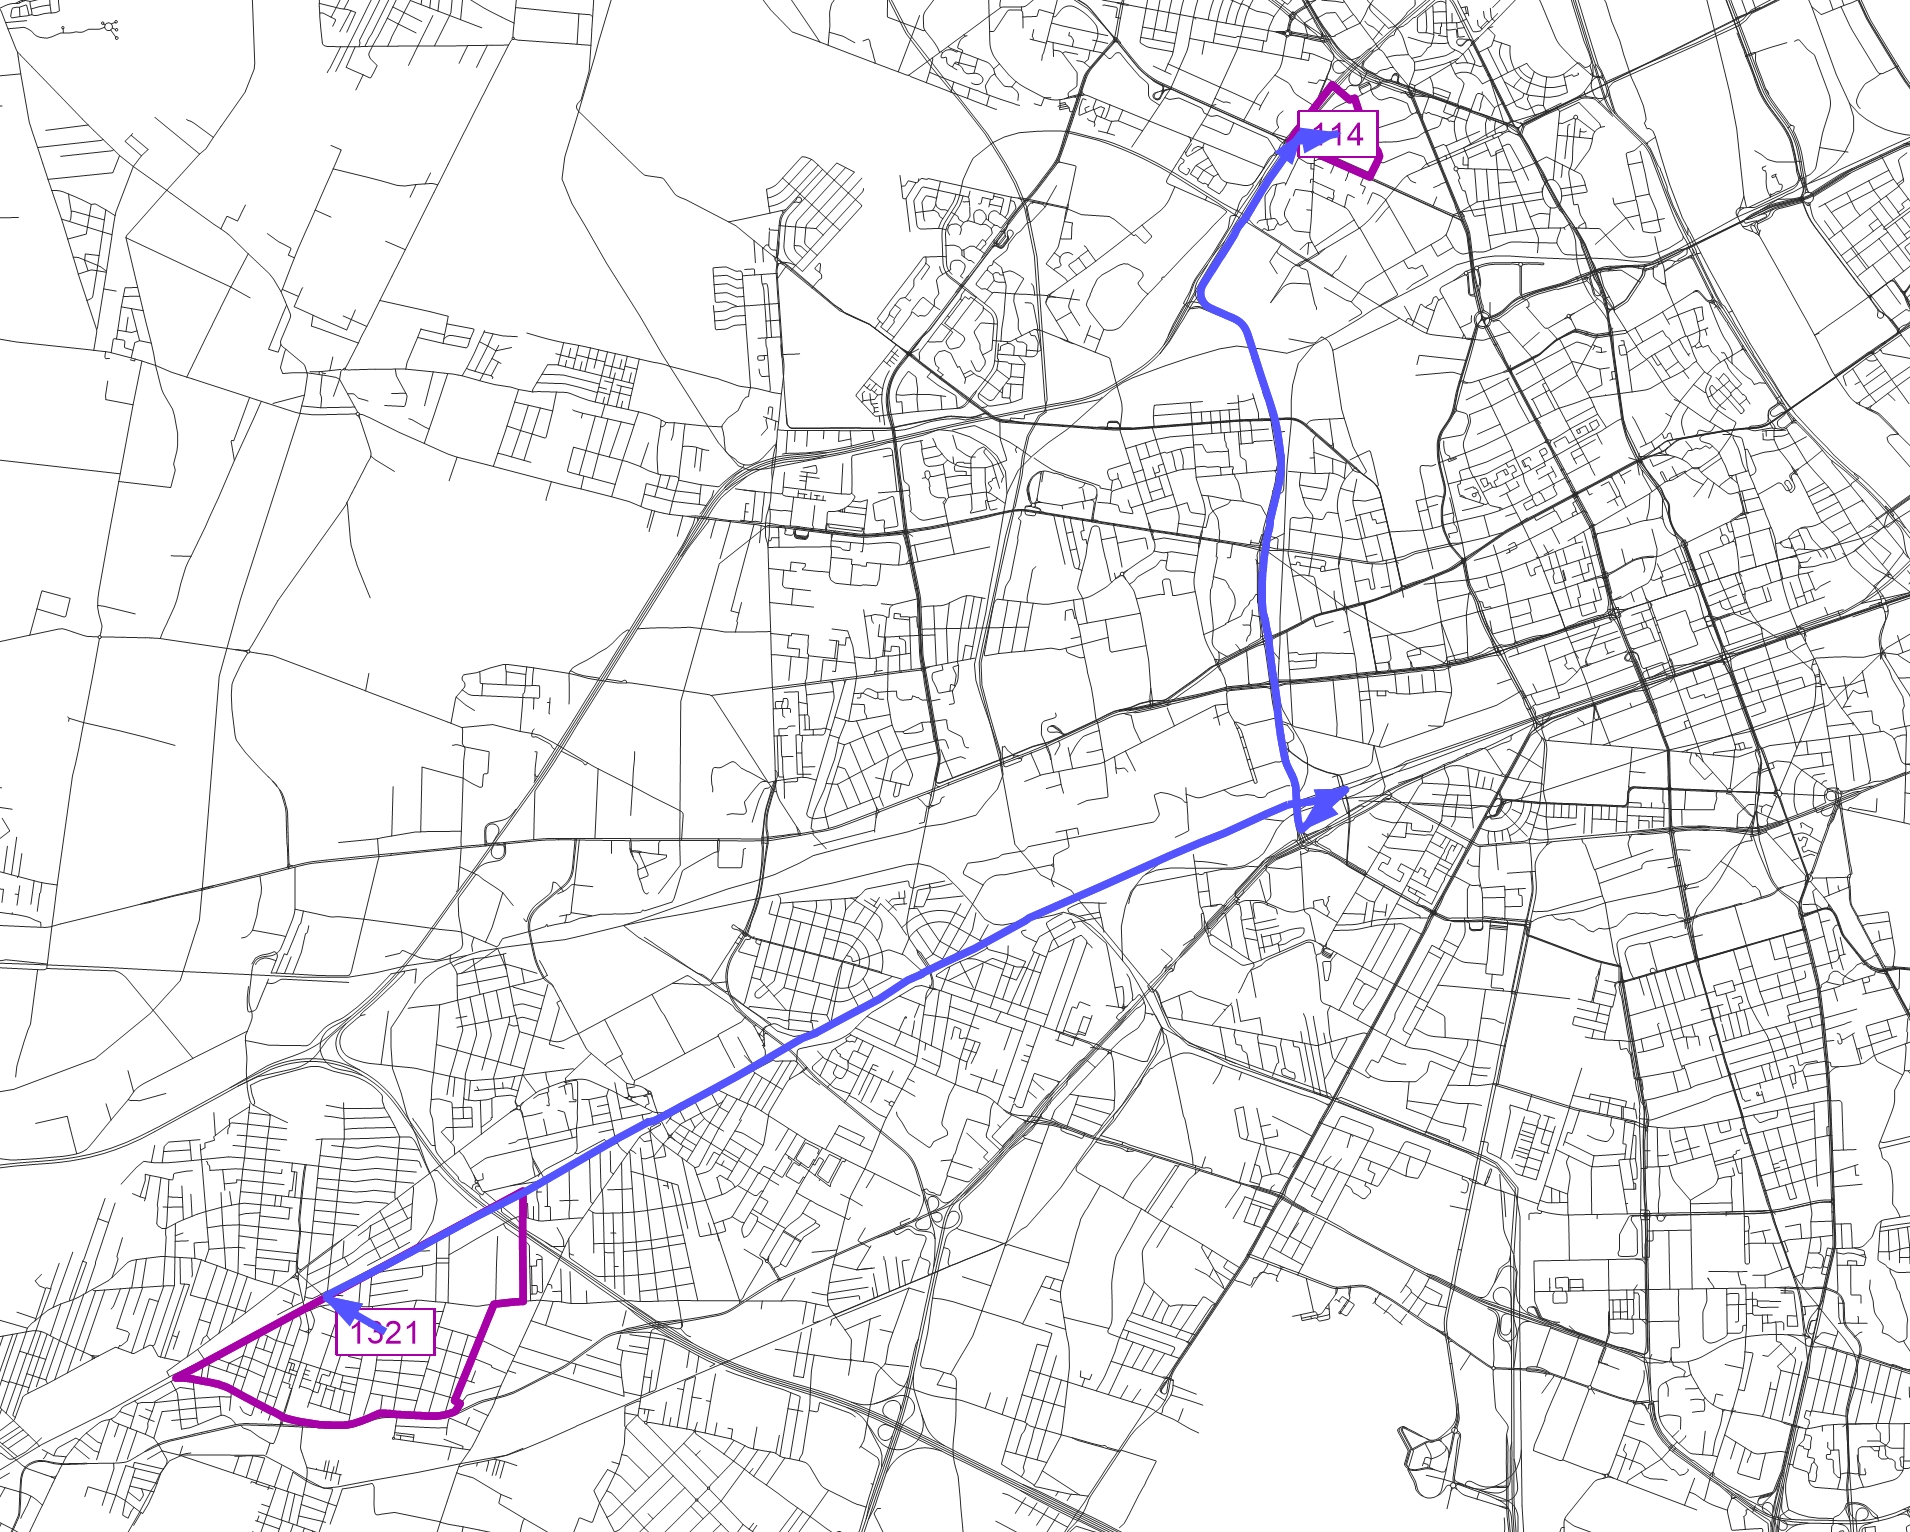
\includegraphics[width=0.8\textwidth]{path_transit}
 \end{center}  \end{figure} 
\end{frame}

\begin{frame}{Shortest paths}{Transit late evening}
\begin{figure}\begin{center}
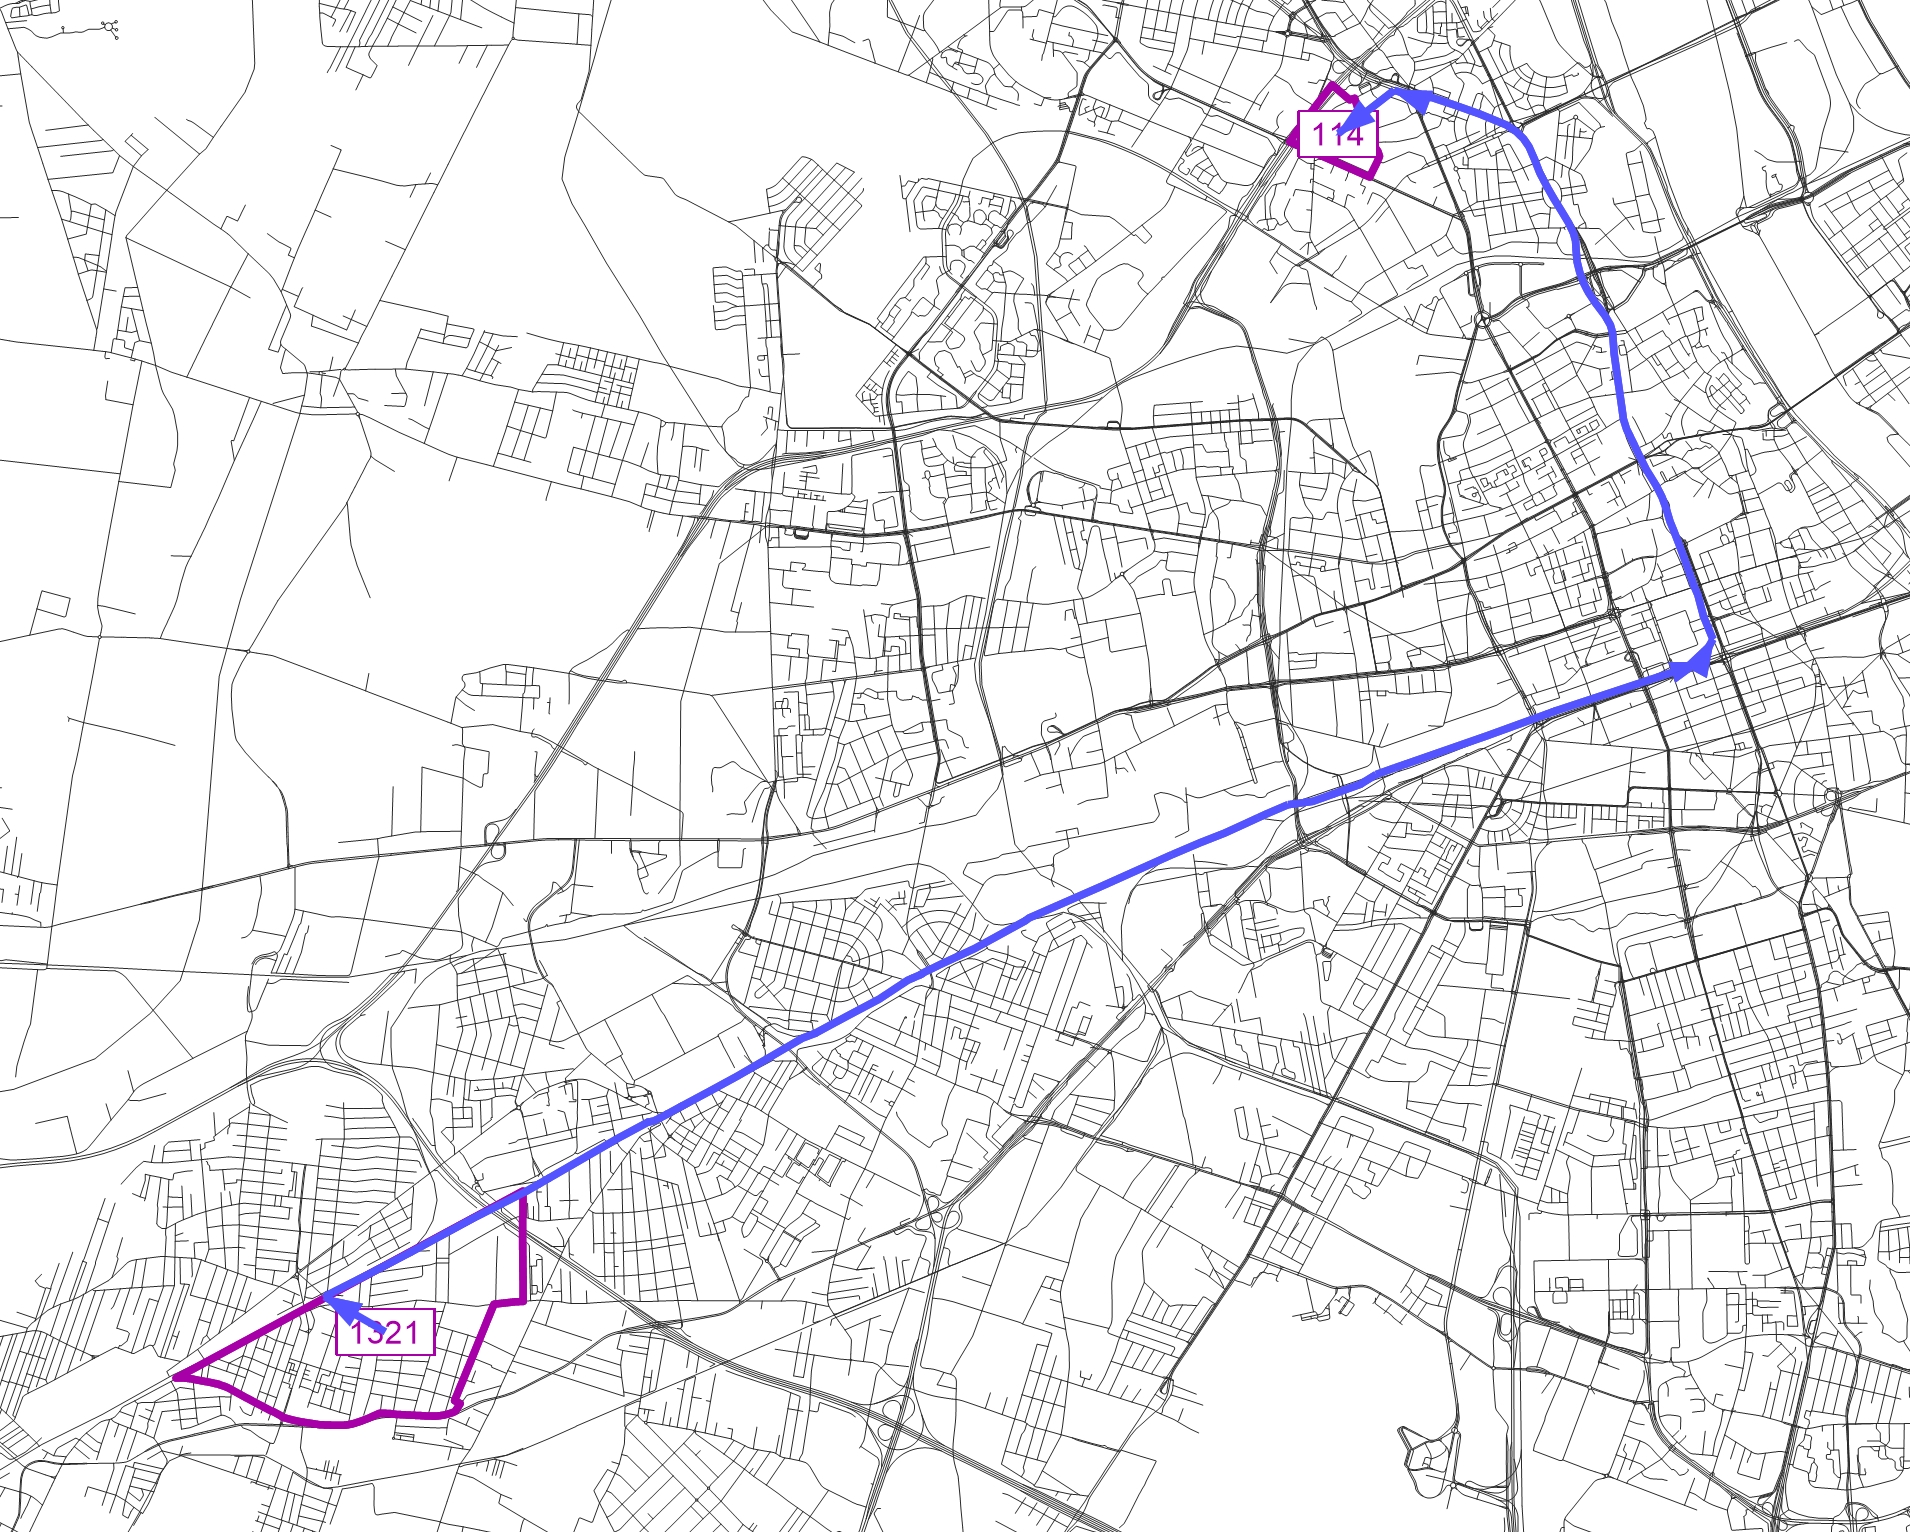
\includegraphics[width=0.8\textwidth]{path_transit2}
 \end{center}  \end{figure} 
\end{frame}


\begin{frame}{Summary}{Thanks for attention}
Rafal Kucharski, rkucharski(at)pk.edu.pl
\end{frame}

\end{document}



